%---------- Inleiding ---------------------------------------------------------

\section{Introductie} % The \section*{} command stops section numbering
\label{sec:introductie}
Hier introduceer je werk. Je hoeft hier nog niet te technisch te gaan.

Je beschrijft zeker:

\begin{itemize}
  \item de probleemstelling en context
  \item de motivatie en relevantie voor het onderzoek
  \item de doelstelling en onderzoeksvraag/-vragen
\end{itemize}
Het uirollen en schalen van applicaties word meer en meer gedaan met behulp van containers en container orcherstratie tools.  
Deze zorgen ervoor dat de ontwikkeling en het uitrollen van een applicatie vergemakkelijkt word. In traditionele 
Gartner (\textcite{Gartner2019})  voorspeld dat tegen 2022 maar liefst 75\% van alle internatiale organisaties gecontaineriseerde applicaties zullen gebruiken in hun productieomgeving.


%---------- Stand van zaken ---------------------------------------------------

\section{State-of-the-art}
\label{sec:state-of-the-art}

Hier beschrijf je de \emph{state-of-the-art} rondom je gekozen onderzoeksdomein. Dit kan bijvoorbeeld een literatuurstudie zijn. Je mag de titel van deze sectie ook aanpassen (literatuurstudie, stand van zaken, enz.). Zijn er al gelijkaardige onderzoeken gevoerd? Wat concluderen ze? Wat is het verschil met jouw onderzoek? Wat is de relevantie met jouw onderzoek?

Verwijs bij elke introductie van een term of bewering over het domein naar de vakliteratuur, bijvoorbeeld~\autocite{kohgadai2020}! Denk zeker goed na welke werken je refereert en waarom.

% Voor literatuurverwijzingen zijn er twee belangrijke commando's:
% \autocite{KEY} => (Auteur, jaartal) Gebruik dit als de naam van de auteur
%   geen onderdeel is van de zin.
% \textcite{KEY} => Auteur (jaartal)  Gebruik dit als de auteursnaam wel een
%   functie heeft in de zin (bv. ``Uit onderzoek door Doll & Hill (1954) bleek
%   ...'')

Je mag gerust gebruik maken van subsecties in dit onderdeel.

%---------- Methodologie ------------------------------------------------------
\section{Methodologie}
\label{sec:methodologie}

Hier beschrijf je hoe je van plan bent het onderzoek te voeren \footnote{"https://molecule.readthedocs.io"} \autocite{Gartner2019}. 
Welke onderzoekstechniek ga je toepassen om elk van je onderzoeksvragen te beantwoorden? Gebruik je hiervoor experimenten, vragenlijsten,
 simulaties? Je beschrijft ook al welke tools je denkt hiervoor te gebruiken of te ontwikkelen.
Voor dit onderzoek zullen er enkele scenario's opgezet worden. Bij elke scenario zullen er verschillende security best practices en security tools gebruikt worden.
Deze zullen getest worden op basis van de volgende criteria: \newline
\begin{itemize}
	\item Deployment snelheid
	\item Benodigde resources
	\item Stabiliteit \newline
\end{itemize} 
Voorbeelden van scenario's: \newline
\begin{itemize}
	\item S(0): Er word een container applicatie opgezet in een Kubernetes cluster zonder extra security configuratie.
	\item S(1): Er word een container applicatie opgezet in een Kubernetes cluster en enkele 'best practices' worden toegepast.
	\item S(2): Er word een container applicatie opgezet in een Kubernetes cluster waarin de grootste security risico's worden vermeden. \newline
\end{itemize} 
Door gebruik te maken van deze scenario's en criteria hopen we te kunnen aanwijzen dat het toepassen van security 'best practices' een positieve invloed heeft op het gebruik van containers en container orcherstratie tools.
%---------- Verwachte resultaten ----------------------------------------------
\section{Verwachte resultaten}
\label{sec:verwachte_resultaten}

Hier beschrijf je welke resultaten je verwacht. Als je metingen en simulaties uitvoert, kan je hier al mock-ups maken van de grafieken samen met de verwachte conclusies. Benoem zeker al je assen en de stukken van de grafiek die je gaat gebruiken. Dit zorgt ervoor dat je concreet weet hoe je je data gaat moeten structureren.
Op basis van de criteria word er verwacht dat Scenario 0 en 1 even snel op gedeployed kunnen worden maar ze zullen wel beide kwetsbaar zijn aangezien de 'best practices' vooral bestaan uithet correct gebruik wachtwoorden en gebruiker privileges.
Scenario 2 daarintegen zal iets meer tijd nodig hebben om te deployen en zal ook meer resources gebruiken. Dit zal vooral komen omdat het delen van resources tussen de containers een security risico is en dus tot een minimum zal moeten beperkt worden.\autocite{Education2019} 
\begin{figure}[ht]
	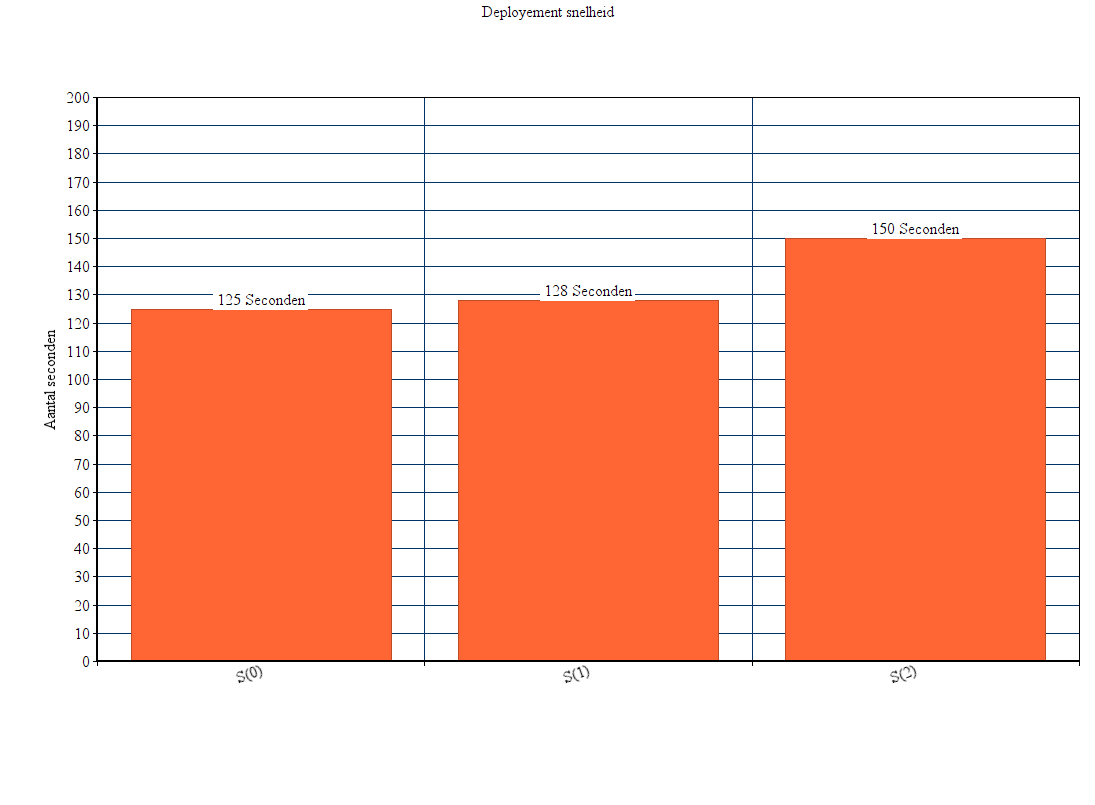
\includegraphics[scale=0.27]{img/Mock1.png}
	\caption{Verwacht eindresultaat}
	\label{fig:example}
	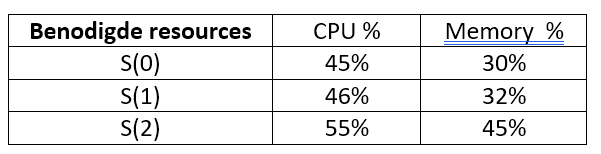
\includegraphics[scale=0.50]{img/Mock2.png}
	\caption{Verwacht eindresultaat}
  \label{fig:example}
\end{figure}
%---------- Verwachte conclusies ----------------------------------------------
\section{Verwachte conclusies}
\label{sec:verwachte_conclusies}

Hier beschrijf je wat je verwacht uit je onderzoek, met de motivatie waarom. Het is \textbf{niet} erg indien uit je onderzoek andere resultaten en conclusies vloeien dan dat je hier beschrijft: het is dan juist interessant om te onderzoeken waarom jouw hypothesen niet overeenkomen met de resultaten.

Uit dit onderzoek verwachten verwachten we te kunnen concluderen dat het toepassen van 'best practices' en het correct gebruik van security tools een positief effect hebben het gebruik van container orcherstratie tools.
We willen ook aanduiden dat het omzeilen van security risico's een belangrijk aspect is bij het developen van container applicaties. 
Tot slot is het mogelijk om de conclusie te trekken dat het beveiligen van container clusters steeds belangrijker word en het ook belangrijk is dat de persoon die een cluster opzet de onderliggende werkwijze goed kent en zich bewust is van de valkuilen.
